%
% pfad.tex
%
% (c) 2017 Prof Dr Andreas Müller, Hochschule Rapperswil
%
\documentclass[tikz]{standalone}
\usepackage{times}
\usepackage{txfonts}
\usepackage{pgfplots}
\usepackage{csvsimple}
\usetikzlibrary{arrows,intersections}
\begin{document}
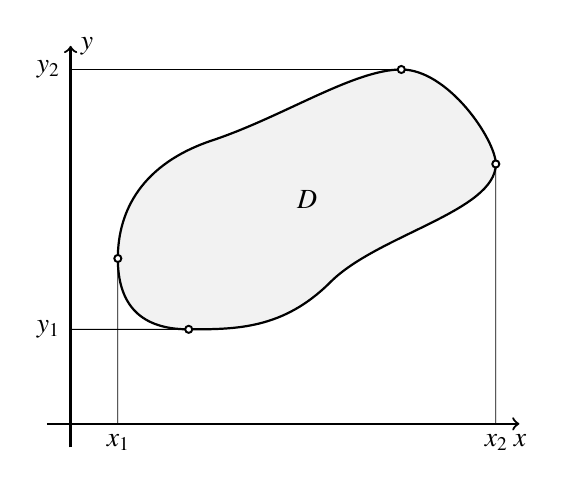
\begin{tikzpicture}[thick,scale=0.3]
\coordinate (O) at (0,0);

\coordinate (A) at ( 5, 4);
\coordinate (B) at (11, 6);
\coordinate (C) at (18,11);
\coordinate (D) at (14,15);
\coordinate (E) at ( 6,12);
\coordinate (F) at ( 2, 7);

\draw[fill=gray!10]	(A) .. controls (7,4) and (9,4) ..
	(B) .. controls (13,8) and (18,9) ..
	(C) .. controls (18,12) and (16,15) ..
	(D) .. controls (12,15) and (9,13) ..
	(E) .. controls (3,11) and (2,9) ..
	(F) .. controls (2,5) and (3,4) ..
	(A);

\node at (10,9.5) {$D$};

\draw[->] (-1,0)--(19,0) coordinate[label = {below:$x$}];
\draw[->] (0,-1)--(0,16) coordinate[label = {right:$y$}];

\draw[line width=0.3] (F)--(2,0);
\draw[line width=0.3] (C)--(18,0);

\draw[line width=0.3] (D)--(0,15);
\draw[line width=0.3] (A)--(0,4);

\node at (0,4) [left] {$y_1$};
\node at (0,15) [left] {$y_2$};

\node at (2,0) [below] {$x_1$};
\node at (18,0) [below] {$x_2$};

\draw[line width=0.7,fill=white] (A) circle[radius=0.15] {};
\draw[line width=0.7,fill=white] (D) circle[radius=0.15] {};
\draw[line width=0.7,fill=white] (C) circle[radius=0.15] {};
\draw[line width=0.7,fill=white] (F) circle[radius=0.15] {};

%\draw[line width=0.2,red]
%	(F) .. controls (2,5) and (3,4) ..
%	(A) .. controls (7,4) and (9,4) ..
%	(B) .. controls (13,8) and (18,9) ..
%	(C);
%
%\draw[blue,line width=0.2]
%	(C) .. controls (18,12) and (16,15) ..
%	(D) .. controls (12,15) and (9,13) ..
%	(E) .. controls (3,11) and (2,9) ..
%	(F);
%
%\node at (B) [below right,red] {$y_1(x)$};
%\node at (E) [above,blue] {$y_2(x)$};
%
%\node at (C) [right,blue] {$x_2(y)$};
%\node at (F) [left,red] {$x_1(y)$};
%
%\draw[red,line width=0.2]
%	(D) .. controls (12,15) and (9,13) ..
%	(E) .. controls (3,11) and (2,9) ..
%	(F) .. controls (2,5) and (3,4) ..
%	(A);
%
%\draw[blue,line width=0.2]
%	(A) .. controls (7,4) and (9,4) ..
%	(B) .. controls (13,8) and (18,9) ..
%	(C) .. controls (18,12) and (16,15) ..
%	(D);

\end{tikzpicture}
\end{document}

